% 12-34(12쪽) — 34~39번 공통 그림 · y=f(x) 의 그래프(x=-1, x=1 에서 빈 점·채운 점 · 안내 점선). 스캔 화질이 낮아 TikZ 로 다시 그림.
% 원문에 있는 것만: 눈금 -1, 1, 2 · y축 옆 1, -1 · 점선 네 줄 · 빈 점 (-1,1), (1,1), (-1,-1) · 채운 점 (-1,0), (1,0) · 라벨 y=f(x), O, x, y.
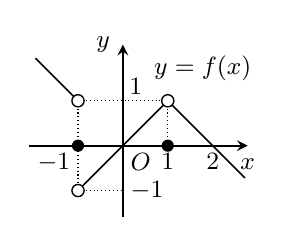
\begin{tikzpicture}[x=0.57cm, y=0.57cm, line width=0.6pt]
  \draw[->, >=stealth, line width=0.7pt] (-2.1,0) -- (2.78,0) node[below=1pt, font=\small] {$x$};
  \draw[->, >=stealth, line width=0.7pt] (0,-1.6) -- (0,2.25) node[left=1pt, font=\small] {$y$};
  \draw[densely dotted, line width=0.4pt] (-1,1) -- (1,1);
  \draw[densely dotted, line width=0.4pt] (-1,1) -- (-1,-1);
  \draw[densely dotted, line width=0.4pt] (1,1) -- (1,0);
  \draw[densely dotted, line width=0.4pt] (-1,-1) -- (0,-1);
  \draw[line width=0.6pt] (-1.95,1.95) -- (-1,1);
  \draw[line width=0.6pt] (-1,-1) -- (1,1);
  \draw[line width=0.6pt] (1,1) -- (2.72,-0.72);
  \draw[fill=white, line width=0.5pt] (-1,1) circle (2.2pt);
  \draw[fill=white, line width=0.5pt] (1,1) circle (2.2pt);
  \draw[fill=white, line width=0.5pt] (-1,-1) circle (2.2pt);
  \fill (-1,0) circle (2.2pt);
  \fill (1,0) circle (2.2pt);
  \node[font=\small, inner sep=2.5pt, below left] at (-1,0) {$-1$};
  \node[font=\small, inner sep=2.5pt, below] at (1,0) {$1$};
  \node[font=\small, inner sep=2.5pt, below] at (2,0) {$2$};
  \node[font=\small, inner sep=2.5pt, below right] at (0,0) {$\pt{O}$};
  \node[font=\small, inner sep=2pt, above right] at (0,1) {$1$};
  \node[font=\small, inner sep=2.5pt, right] at (0,-1) {$-1$};
  \node[font=\small, inner sep=1pt] at (1.78,1.72) {$y=f(x)$};
\end{tikzpicture}
